
\section{ Question 4:Atmospheres }\label{sec:q4}    


\textbf{(a)}As the bond albedo depends on the reflected flux of the planet, this flux can vary derpending on its composition, cloud coverage or the structure of its athmosphere. Thus, the bond and geometric albedo of a planet are within a given range.

\textbf{(b)} Equilibrium temperature ranges: 

\begin{equation}
T = \frac{1-A_B}{4\epsilon\sigma}\frac{F}{d^2} = 1.38\e{6}, 3.011\e{6}
\end{equation}


\textbf{(c)}Cloud coverage and green house effect as, for example, Venus. (Radiation is reflected by the CO2 gas). Ice greenhouse effect can happen in the Icy Galilean Moons, where the ice reflects the radiation. Finally, dust storms, as for example in Mars. ii) Not sure about this one, it might be ice greenhouse effect at Triton is covered by ice.


\textbf{(d)} 1 If we draw line A of Figure 2 in the Figure 1, we observe that it crosses the profile of each giant at a lower altitude. 2 Same as before, we only have to put the range of line C in Figure 1 and see where they cross: moreorless in 5 bars.

\textbf{(e)} Figure 4.9 Book. While covered by clouds, the absorption lines are shallower.

\begin{figure}
	\centering
	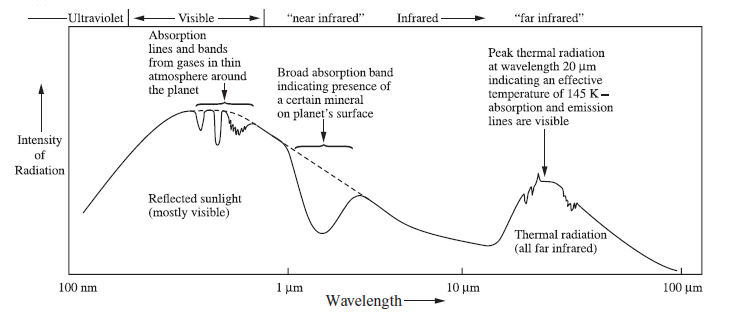
\includegraphics[width=0.7\linewidth]{pics/Q4}
	\caption{}
	\label{fig:q4}
\end{figure}